\section{Reciprocal Lattices}

\begin{parts}
\item The reciprocal lattice of a 1D lattice with lattice constant $a$ is defined simply by

  \begin{equation}
    G = m\left(\frac{2\pi}{a} \right).
  \end{equation}

  \begin{figure}
    \centering
    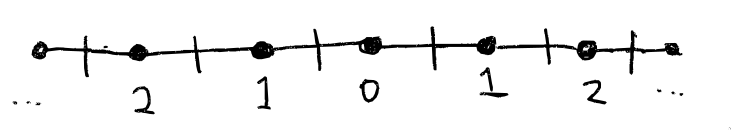
\includegraphics[width=0.6\linewidth]{./res/Pics/4-a.png}
    \caption{}\label{fig:4-a}
  \end{figure}

  I have drawn a picture of what this looks like in Fig.~\ref{fig:4-a}, where the distance between reciprocal lattice points is given by $(2\pi/a)$. We can pretty easily determine a relation for the $n$th Brillouin zone:

  \begin{equation}
    - \frac{2n\pi}{a} \leq G < - \frac{2(n-1)\pi}{a} \ \cup \ \frac{2(n-1)\pi}{a} \leq G < \frac{2n\pi}{a}.
  \end{equation}



\item We know that the relation between the primitive reciprocal lattice vectors and the primite lattice vectors is given by

  \begin{equation}
    \vv{g}_i = 2\pi \frac{\vv{a}_j \times \vv{a}_k}{|(\vv{a}_1 \times \vv{a}_2| \cdot \vv{a}_3}.
  \end{equation}

  If we dot this with a primitive lattice vector $\vv{a}_\ell$, we get

  \begin{equation}
    \vv{a}_\ell \cdot \vv{g}_i = 2\pi \frac{\vv{a}_\ell (\vv{a}_j \times \vv{a}_k)}{|(\vv{a}_1 \times \vv{a}_2| \cdot \vv{a}_3}.
  \end{equation}

  The cross product between two vectors yields a new vector that is perpendicular to both original vectors. A therefore, the dot product in the numerator is only satisfied when $\ell=i$, which leads is simply the volume of the unit cell in real space, $\Omega_p$. Therefore,

  \begin{equation}
    \vv{a}_\ell \cdot \vv{g}_i = 2\pi \delta_{\ell,i}.
  \end{equation}

  Dotting the full reciprocal and real lattice vectors we therefore find

  \begin{equation}
    \vv{G}_m \cdot \vv{R}_n = 2\pi \sum_i m_nn_i \equiv 2\pi\nu.
  \end{equation}



\item The primitive lattice vectors for a FCC lattice are

  \begin{equation}
    \vv{a}_1 = \frac{a}{2}(\vh{y} + \vh{z}),\ \vv{a}_2 = \frac{a}{2}(\vh{z} + \vh{x}),\ \text{and}\ \vv{a}_3 = \frac{a}{2}(\vh{x} + \vh{y}).
  \end{equation}

  We will need the cross products of these vectors to continue. First,

  \begin{equation}
    \vv{a}_1 \times \vv{a}_2 = \frac{a^2}{4} \begin{vmatrix} \vh{x} & \vh{y} & \vh{z} \\ 0 & 1 & 1 \\ 1 & 0 & 1 \end{vmatrix} = \frac{a^2}{4}(\vh{x} + \vh{y} - \vh{z}).
  \end{equation}

  Since the $\vv{a}$ vectors are cyclic, so too will these cross products. Now, the area of the real-space unit cell $\Omega_p$ is given by

  \begin{equation}
    \Omega_p = (\vv{a}_1 \times \vv{a}_2) \cdot \vv{a}_3 = \frac{a^3}{8}(\vh{x} + \vh{y} - \vh{z})\cdot(\vh{x} + \vh{y}) = \frac{a^3}{4}.
  \end{equation}

  Therefore,

  \begin{equation}
    \vv{g}_1 = 2\pi \frac{4}{a^3} \cdot \frac{a^2}{4} (\vv{a}_2 \times \vv{a}_3) = \frac{2\pi}{a} (-\vh{x} + \vh{y} + \vh{z}).
  \end{equation}

  Again, since the cross products of the $\vv{a}$ vectors are cyclic, we can go ahead and find that

  \begin{align}
    \vv{g}_2 &= \frac{2\pi}{a} (\vh{x} - \vh{y} + \vh{z}),\ \text{and} \\
    \vv{g}_3 &= \frac{2\pi}{a} (\vh{x} + \vh{y} - \vh{z}).
  \end{align}

  These are directly proportional to the primitive lattice vectors for the BCC lattice; hence, the reciprocal lattice of the FCC lattice is a BCC lattice in reciprocal space.

  We now will show the inverse of the above statement; i.e. that the reciprocal lattice of the BCC lattice is an FCC lattice in reciprocal space. Following the same steps, we need the cross products of the BCC primitive lattice vectors:

  \begin{equation}
    \vv{a}_1 \times \vv{a}_2 = \frac{a^2}{4} \begin{vmatrix} \vh{x} & \vh{y} & \vh{z} \\ -1 & 1 & 1 \\ 1 & -1 & 1 \end{vmatrix} = \frac{a^2}{2}(\vh{x} + \vh{y}).
  \end{equation}

  These are cyclic for the same reason as with the previous part. So,

  \begin{equation}
    \Omega_p = \frac{a^2}{4}(\vh{x} + \vh{y}) \cdot (\vh{x} + \vh{y} - \vh{z}) = \frac{a^3}{2}.
  \end{equation}

  We can now find

  \begin{equation}
    \vv{g}_1 = 2\pi \frac{2}{a^3} \frac{a^2}{4} (\vv{a}_2 \times \vv{a}_3) = \frac{2\pi}{a} \cdot \frac{2}{a^2} \cdot \frac{a^2}{2}(\vh{y} + \vh{z}) = \frac{2\pi}{a}(\vh{y} + \vh{z}), 
  \end{equation}

  so

  \begin{align}
    \vv{g}_2 &= \frac{2\pi}{a}(\vh{z} + \vh{x}),\ \text{and} \\
    \vv{g}_3 &= \frac{2\pi}{a}(\vh{x} + \vh{y}).
  \end{align}

  These are proportional to the primitive lattice vectors for the FCC lattice.



\item We have the identity (in any dimension)

  \begin{equation}
    \vv{G}_{\vv{m}} \cdot \vv{R}_{\vv{n}} = 2\pi\nu,\ \nu\in\mathbb{Z}.
  \end{equation}

  where $\vv{G}_{\vv{m}}$ is a reciprocal lattice vector. If we consider a $\vv{V}_{\vv{n}'}$ in the reciprocal space of $\vv{G}$, we must also have the condition

  \begin{equation}
    \vv{V}_{\vv{n}'} \cdot \vv{G}_{\vv{m}} = 2\pi\nu',\ \nu'\in\mathbb{Z}.
  \end{equation}

  However, since the dot product is commutative, this is saying that $\vv{V}_{\vv{n}'}$ is proportional to $\vv{R}_{\vv{n}}$ up to an integer (which itself is proportional to $n$), meaning that $\vv{V}_{\vv{n}'}$ is an element of the original lattice. Hence, the reciprocal space of the reciprocal space of a lattice comes back to the real space of the lattice.

  
  
\end{parts}


%%% Local Variables:
%%% mode: LaTeX
%%% TeX-master: "../../HW3"
%%% End:
